\section{Introduction}
The architecture of the IPOL demo system is a SOA\footnote{Service-Oriented Architecture.} based on microservices. This change was motivated by the problems found in the previous version of the demo system. First, it was designed as a monolithic program\footnote{Of course, with a good separation of functionality among different classes.} which made it quite easy to deploy in the servers and to run it locally, but at the cost of many disadvantages.
%
Given that it was a monolithic system, it was difficult to split it into different machines to share the computational load of the algorithms being executed. A simple solution would be to create specialized units to run the algorithms and to call them from the monolithic code, but this clearly evokes the first step to move to a microservices architecture. Indeed, this first step of \emph{breaking the monolith}~\cite{neuman2015building} can be iterated until all the functions of the system have been delegated in different modules. In the case of IPOL, we created specialized modules and removed the code from the monolith until the very monolith became a module itself: the Core. This Core module is in charge of all the system and delegates the operations to other modules. Fig. \ref{fig:architecture} summarizes the IPOL modules and other components of the system.

\begin{figure}[!ht]
\centering
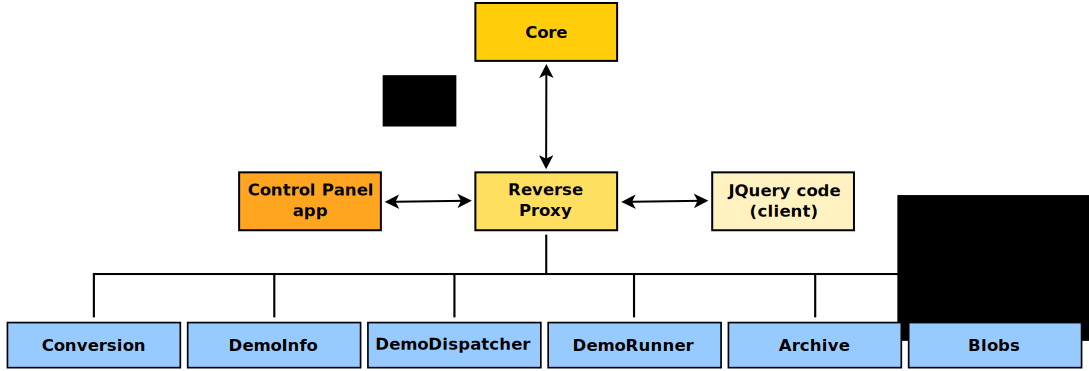
\includegraphics[width=0.8\linewidth]{architecture/images/architecture.pdf}
\caption{The IPOL modular system architecture.} 
\label{fig:architecture}
\end{figure}

Other problems we had in the previous version of the demo system got solved when we moved to the microservices architecture. Since there is a loose coupling between the Core and the other modules, different members of the development team can work at the same time without worrying about the implementation details or data structures used in other parts of the system. Also, tracking down malfunctions is easier: since the Core centralizes all the operations, when a bug shows it can only be generated either at the Core or at the involved module, but not at any other part of the system. In the old system a bug could be caused by complex conditions which depend on the global state of the program, making debugging a complex task. And as noted before, the fact that the architecture of the system is distributed and modular by design makes it very natural and simple to have mechanisms to share the computational load among several machines.

Hiding the internal implementation details behind the interfaces of the modules is an essential part of the system, and it is needed to provide loose coupling between its components. The internal architecture of the system is of course hidden from the users when they interact with the system, but it is also hidden \emph{from the inside}. This means that any module (the Core included) does not need to know the location of the modules. Instead, all of them use a published API.

Once the API is defined, the routing to the modules is implemented by a reverse proxy. It receives the requests from the clients according to this pattern: \verb|/api/<module>/<service>| and redirects them to the corresponding module. Fig. \ref{fig:reverse_proxy} shows how the API messages received by the proxy are routed to the corresponding modules, thus hiding the internal architecture of the system.

\begin{figure}[!ht]
    \centering
    \includegraphics[width=0.8\columnwidth]{proxy/images/reverse_proxy.pdf}
    \caption{The reverse proxy routes the API messages to the corresponding modules.}
    \label{fig:reverse_proxy}
\end{figure}

